\documentclass{article}

\usepackage[english]{babel}

% Set page size and margins
\usepackage[a4paper,top=2cm,bottom=2cm,left=3cm,right=3cm,marginparwidth=1.75cm]{geometry}

% Useful packages
\usepackage{amsmath}
\usepackage{graphicx}
\usepackage[colorlinks=true, allcolors=blue]{hyperref}


\title{(Seq2SQL)Sequence to SQL Query with Neural Networks}

\begin{document}
\maketitle

\begin{table}[h]
    \centering
    \begin{tabular}{ll}
        Registration number: & \textcolor{red}{2111046}\\
        Project: & \textcolor{red}{Seq2seq translation}\\
        Link to GitHub: & \url{https://github.com/JJEEEFFFF}\\
    \end{tabular}
\end{table}



\begin{table}[h]
    \centering
    \begin{tabular}{lc}
        Executive summary (max.\ 250 words) & \textcolor{red}{153}\\
        Introduction (max.\ 600 words) & \textcolor{red}{299}\\
        Data (max.\ 500 words/dataset) & \textcolor{red}{87}\\
        Methodology (max.\ 600 words) & \textcolor{red}{488}\\
        Conclusions (max.\ 500 words) & \textcolor{red}{61}\\
        \hline
        Total word count & \textcolor{red}{1088}\\
    \end{tabular}
    %\caption{Word counts for each section.}
\end{table}

\tableofcontents

\clearpage



\begin{abstract}
Sequence to Sequence Translation in simple words is changing a given statement(Interactive Natural language) to computer language and to give back the target statement(SQL Query). To achieved excellent performance on difficult learning tasks a powerful model called Deep Neural Networks (DNNs) are used. Although DNNs work well, whenever
large labeled training sets are available, they cannot be used to map sequences to
SQL Queries.

In this paper we are going to try using different methods to convert the source statement(Interactive Natural language) to the Target statement(SQL queries). To analyse the limitations of sequence to SQL translations, the first method we going to use in this paper is a multilayered Long Short-Term Memory (LSTM) to map the input sequence(INL)
to a vector of a fixed dimension, and then another deep LSTM to decode the
target sequence (SQL) from the vector. We will also be trying out different approaches.

\end{abstract}


\section{Introduction}

Sequence to Sequence translation has various approaches in the recent years, using Neural Networks is one of the most efficient way to achieve the target statement from the source statement. Deep Neural Networks (DNNs) are extremely powerful machine learning models that achieve excellent performance on difficult problems such as speech recognition [13, 7] and visual object recognition [19, 6, 21, 20]. DNNs are powerful because they can perform arbitrary parallel computation
for a modest number of steps. A surprising example of the power of DNNs is their ability to sort
N N-bit numbers using only 2 hidden layers of quadratic size [27]. So, while neural networks are
related to conventional statistical models, they learn an intricate computation.

Relational databases store a significant amount of the worlds data and provide the foundation of many applications in medical, finance and many other sectors. Understanding of query languages such as SQL is required to access relational databases, which is difficult to
master. Natural language interfaces (NLI), a research area at the intersection of natural language
processing and human-computer interactions, seeks to provide means for humans to interact with
computers through the use of natural language~\cite{androutsopoulos1995natural}. relational databases: translating natural language questions to
SQL queries.

First, we introduce Seq2SQL, a deep neural
network for translating natural language questions to corresponding SQL queries. Seq2SQL consists of three components that leverage the structure of SQL to prune the output
space of generated queries. Moreover, it uses policy-based reinforcement learning (RL) to generate
the conditions of the query, which are unsuitable for optimization using cross entropy loss due
to their unordered nature. We train Seq2SQL using a mixed objective, combining cross entropy
losses and RL rewards from in-the-loop query execution on a database. These characteristics allow
Seq2SQL to achieve state-of-the-art results on query generation.


\section{Data}

We use spider dataset. Spider is a collection of questions, corresponding SQL queries, and SQL tables. Spider is the largest hand-annotated semantic parsing dataset to date - it is an order of magnitude larger than other datasets that have logical forms, either in terms of the number of examples or the number of tables. The queries in Spider span over a large number of tables and hence presents an unique challenge: the model must be able to not only generalize to new queries, but to new table schema.

Link to the Spider dataset:\url{https://yale-lily.github.io/spider}

\section{Methodology}

Spider task is to generate a SQL query from a natural language question and table schema.
Our baseline model is the attentional sequence to sequence neural semantic parser that achieves state-of-the-art performance on a host of semantic parsing datasets
without using hand-engineered grammar. In particular, we can limit the output space of the generated
sequence to the union of the table schema, question utterance, and SQL key words. We first describe
the augmented pointer network model, then address its limitations in our definition of Seq2SQL,
particularly with respect to generating unordered query conditions.
\clearpage

\begin{figure}[htp]
    \centering
    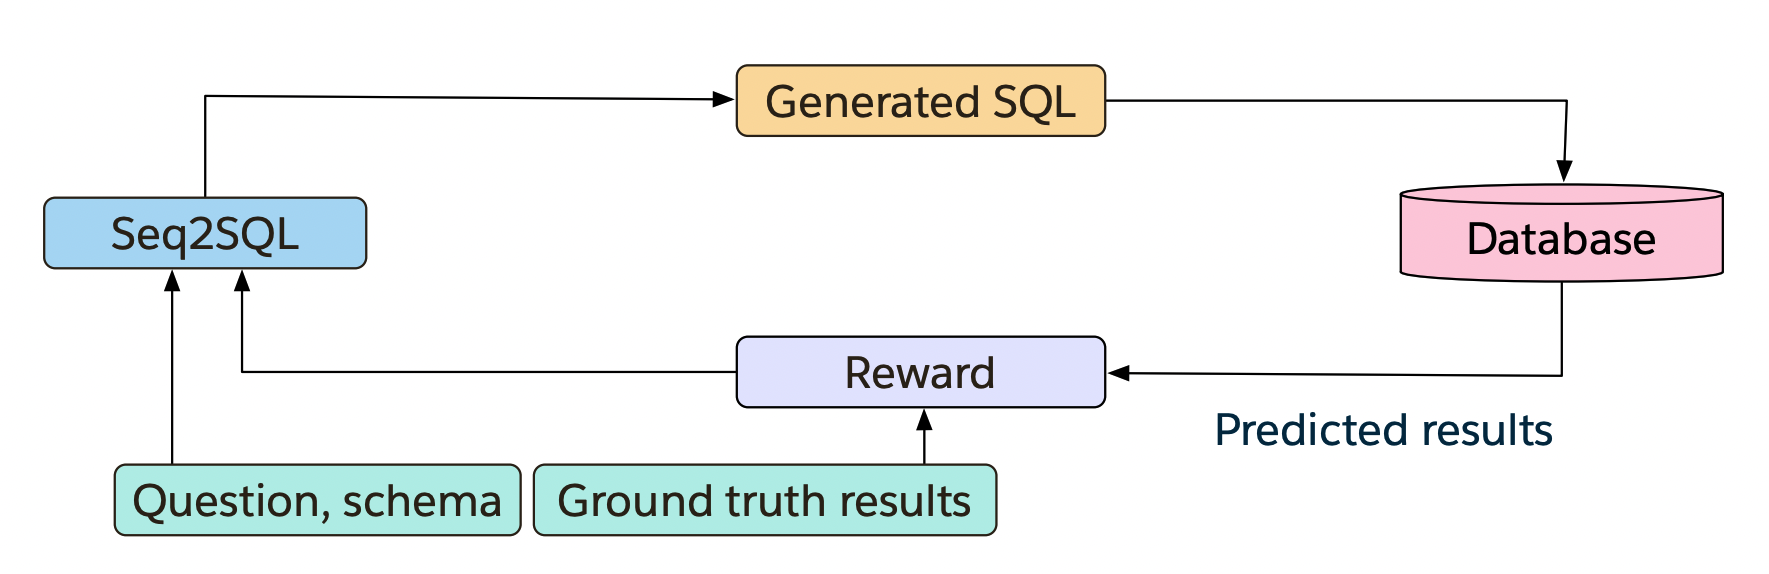
\includegraphics[width=10cm]{Seq2SQL Fig 1}
    \caption{ Seq2SQL takes as input a question and the columns of a table. It generates the corresponding SQL query, which, during training, is executed against a database. The result of the
execution is utilized as the reward to train the reinforcement learning algorithm.}
    \label{fig:galaxy}
\end{figure}

\subsection{AUGMENTED POINTER NETWORK}
The augmented pointer network generates the SQL query token-by-token by selecting from an input
sequence. In our case, the input sequence is the concatenation of the column names, required for the
selection column and the condition columns of the query, the question, required for the conditions
of the query, and the limited vocabulary of the SQL language such as SELECT, COUNT etc. With this augmented input sequence, the pointer network
can produce the SQL query by selecting exclusively from the input.

Suppose we have a list of N table columns and a question such as in Figure 2, and want to produce
the corresponding SQL query. Let x
c
j = [x
c
j,1
, xc
j,2
, ...xc
j,Tj
] denote the sequence of words in the
name of the jth column, where x
c
j,i represents the ith word in the jth column and Tj represents the
total number of words in the jth column. Similarly, let x
q
and x
s
respectively denote the sequence
of words in the question and the set of unique words in the SQL vocabulary. Reference~\cite{zhong2017seq2sql}

\subsection{ SEQ2SQ}


While the augmented pointer network can
solve the SQL generation problem, it does
not leverage the structure inherent in SQL.
Typically, a SQL query consists of three components.
The first component is the aggregation operator, in this case COUNT, which produces a summary of the rows selected by
the query. Alternatively the query may request no summary statistics, in which case
an aggregation operator is not provided.
The second component is the SELECT
column(s), which
identifies the column(s) that are to be included in the returned results. The third
component is the WHERE clause of the query,
which contains conditions by which to filter the rows. The first two components
are supervised using cross entropy loss, whereas the third generation component is trained using
policy gradient to address the unordered nature of query conditions. Utilizing the structure of SQL allows Seq2SQL to further prune
the output space of queries, which leads to higher performance than Seq2Seq and the augmented
pointer network


\section{Conclusions}

We proposed Seq2SQL, a deep neural network for translating questions to SQL queries.To train Seq2SQL,
we applied in-the-loop query execution to learn a policy for generating the conditions of the SQL
query, which is unordered and unsuitable for optimization via cross entropy loss. We show that Seq2SQL outperforms a state-of-the-art semantic parser
on Spider, improving execution accuracy and logical form accuracy.


\bibliographystyle{plain}
\bibliography{bibliography1.bib}
\end{document}